\documentclass[russian]{beamer}
\usepackage{mystyleslides}
\usepackage{cohmystyle}
\usepackage{changepage}

% https://tex.stackexchange.com/questions/1656/footnote-counter-would-like-to-restart-from-1-each-page
% https://stackoverflow.com/questions/3701605/how-to-restart-footnote-numbering-every-page

% \usepackage[perpage]{footmisc}

% \usepackage{perpage}
% \MakePerPage{footnote}

%% \usepackage{eulervm}
%% \usepackage{fourier}

\graphicspath{ {images/} }

\usetheme{Warsaw} % Warsaw Copenhagen Madrid CambridgeUs Darmstadt Frankfurt Singapore
\setbeamertemplate{headline}{}

\definecolor{beamer@blendedblue}{RGB}{13, 74, 76}
%% 0, 65, 106 *
%% 0, 51, 102
%% 8, 69, 126
%% 0, 49, 83

%% 17, 96, 98
%% 1, 58, 51

\definecolor{my-red}{RGB}{176, 0, 0}
\definecolor{my-blue}{RGB}{0, 0, 153}
\definecolor{my-teal}{RGB}{0, 153, 153}
\definecolor{my-green}{RGB}{0, 153, 0}
\definecolor{my-violet}{RGB}{75, 0, 130}
\definecolor{my-pink}{RGB}{253, 123, 124}
%{90, 45, 102} % violet
%{145, 30, 66} % light cherry
%{146, 43, 62} % cherry

%\usecolortheme{default}
%\usecolortheme{sidebartab}
%\usefonttheme{default}

% Inserting frame numbers in footline
% http://tex.stackexchange.com/questions/191198/customization-of-the-copenhagen-theme
\makeatletter
  \iffalse
  \pgfdeclarehorizontalshading[frametitle.bg,frametitle right.bg]{beamer@frametitleshade}{\paperheight}{%
    color(0pt)=(myblue2);
    color(\paperwidth)=(white)}
  \fi

  \defbeamertemplate*{footline}{mysplit theme}
  {%
    \leavevmode%
    \hbox{\begin{beamercolorbox}[wd=.5\paperwidth,ht=2.5ex,dp=1.125ex,leftskip=.3cm plus1fill,rightskip=.3cm]{author in head/foot}%
      \usebeamerfont{author in head/foot}\insertshortauthor
    \end{beamercolorbox}%
    \begin{beamercolorbox}[wd=.5\paperwidth,ht=2.5ex,dp=1.125ex,leftskip=.3cm,rightskip=.3cm plus1fil]{title in head/foot}%
      \usebeamerfont{title in head/foot}\insertshorttitle\hfill
      \insertframenumber\ / \inserttotalframenumber\hspace*{0.5em}
    \end{beamercolorbox}}%
    \vskip0pt%
  }
\makeatother


% https://tex.stackexchange.com/questions/170222/change-the-numbering-in-beamers-table-of-content
%\makeatletter
%\patchcmd{\beamer@sectionintoc}
%  {\ifnum\beamer@tempcount>0}
%  {\ifnum\beamer@tempcount>-1}
%  {}
%  {}
%\beamer@tocsectionnumber=-1
%\makeatother


%\setbeamertemplate{footline}[frame number] % page numbering outside Navigation Bar
\setbeamertemplate{navigation symbols}{} % switch off navigation bar
%\setbeamertemplate{caption}[numbered]

\setbeamertemplate{itemize item}[ball] % Загадка, но без этого у itemize не будет кружочков % itemize items
\setbeamertemplate{itemize subitem}[triangle]
\newcommand{\labelitemi}{\usebeamertemplate{itemize item}{}} % Загадка, но без этого у itemize не будет кружочков
\newcommand{\labelitemii}{\usebeamertemplate{itemize subitem}{}} % https://tex.stackexchange.com/questions/12735/can-one-replace-bullet-points-with-graphics

\iffalse
\AtBeginSection[]
{
  \begin{frame}
    \frametitle{Table of Contents}
    \tableofcontents[currentsection]
  \end{frame}
}
\fi

\title[Внутритекстовая когерентность]
{
  Внутритекстовая когерентность\\
  как мера интерпретируемости\\
  тематических моделей текстовых коллекций\\
}
\subtitle{}

\author[Василий Алексеев]{
  Василий Алексеев
}

\institute[]
{
  \footnotesize
  % MIPT
  % 
\includegraphics[height=1.2cm]{mipt_logo_eng}
}

\date[IS 2018]
{
  \footnotesize
  {
    Предзащита бакалаврской работы\\ \bigskip 13 июня 2018
  }
}

\titlegraphic{
  
\includegraphics[height=1.2cm]{mipt_logo_eng}
% https://tex.stackexchange.com/questions/107340/how-to-shift-graphics-adjust-placement-of-figure-with-includegraphics
}


\iffalse
% https://tex.stackexchange.com/questions/74023/two-logos-in-opposite-side-on-beamer
\logo{%
  \makebox[0.95\paperwidth]{%
    
\includegraphics[width=1cm,keepaspectratio]{dialogue_logo}%
    \hfill%
    
\includegraphics[width=1cm,keepaspectratio]{mipt_logo_eng}%
  }%
}
\fi


\begin{document}
  % \maketitle
  % \thispagestyle{empty}
  % \newpage

  % \pagenumbering{arabic}
		
  % \tableofcontents
  % \newpage

  % \addcontentsline{toc}{section}{Пролог}
  % \include{prologue}
  
\frame{\titlepage}


\begin{frame}{Тема, Интерпретируемость и Когерентность}
  \emph{Тема} характеризуется набором слов, которые часто совместно встречаются в тексте.
  \emph{Топ\=/слова} темы~---~её самые частые слова.
  
  \medskip
  
  \emph{Интерпретируемость} темы означает, может ли человек по словам темы объяснить, о чём она, дать ей подходящее название.
  
  \vspace{0.25cm}
  
  \begin{exampleblock}{Хорошо интерпретируемая тема (самые частые слова)}
    актёр, пьеса, музыкальный, премьера, партер, зритель, продюсер, аудитория, занавес, оркестр
  \end{exampleblock}
  
  \begin{alertblock}{Плохо интерпретируемая тема (самые частые слова)}
    экспресс, эпиграф, туманный, результат, образ, право, 
    заём, иероглиф, лак, футбол
  \end{alertblock}
  
  \smallskip
  
  \emph{Когерентность}~---~это автоматический способ оценки интерпретируемости, когда оценивается, как часто топ\=/слова темы встречаются недалеко друг от друга в тексте.
\end{frame}


\begin{frame}{Проблема подхода к оценке интерпретируемости через совстречаемости топ-слов тем}
  \begin{minipage}{0.70\textwidth}
    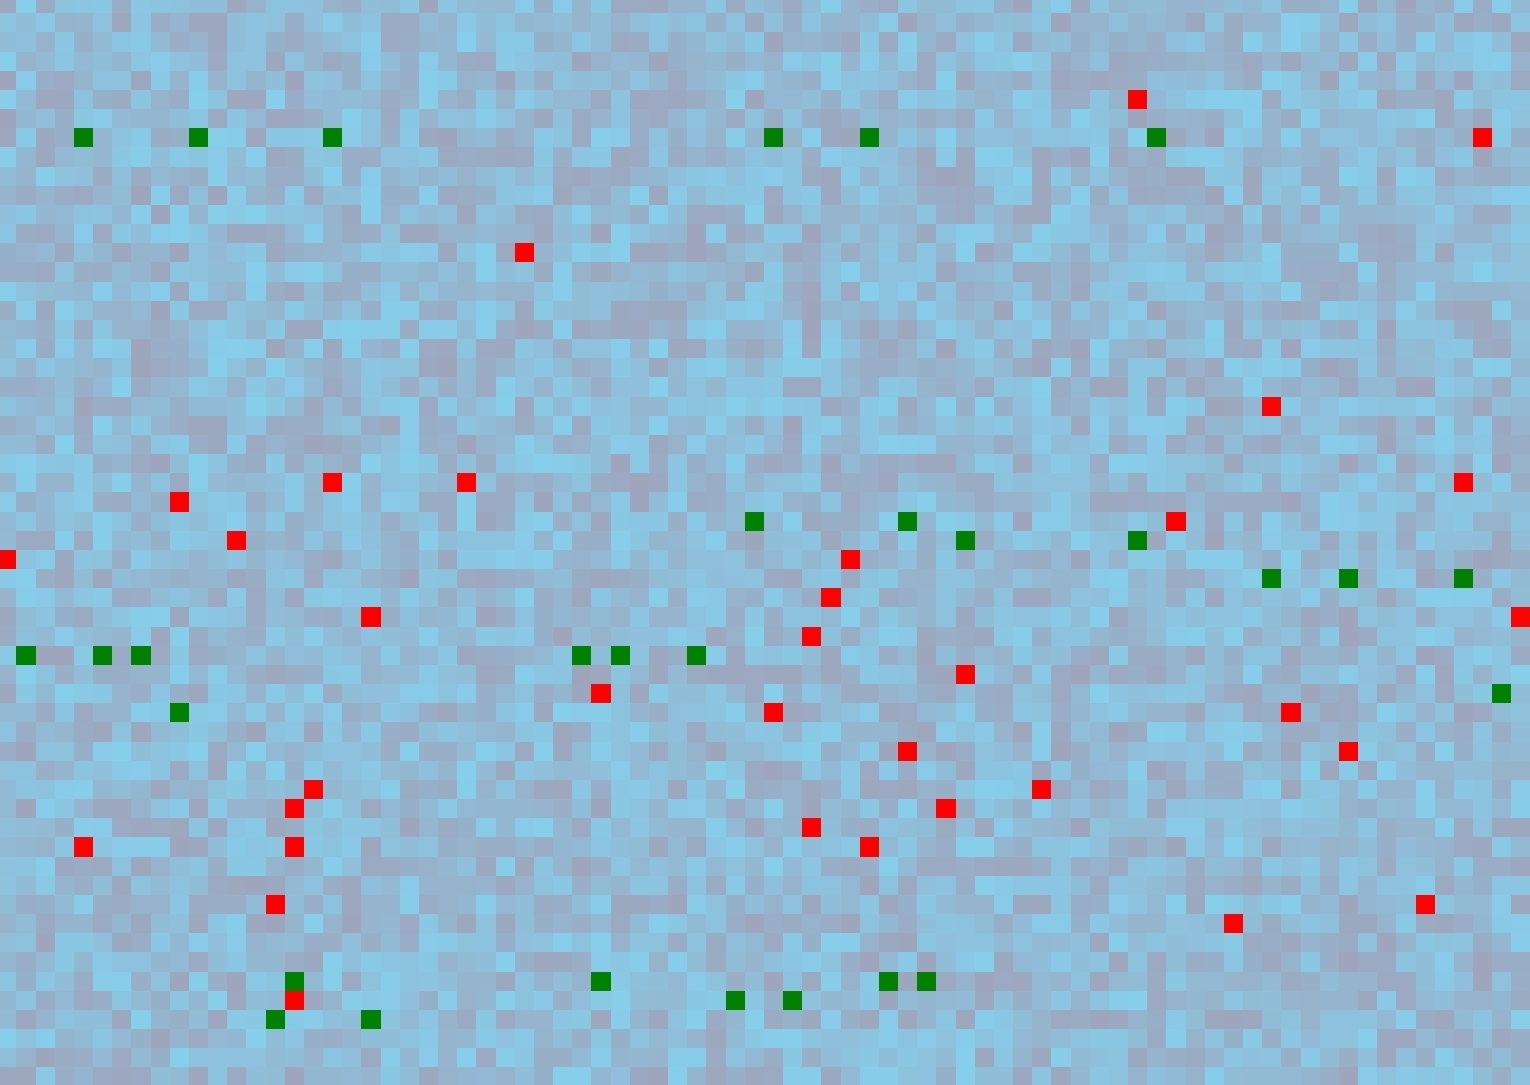
\includegraphics[width=\textwidth]{doc11358_topic0.jpg}
  \end{minipage}
  ~
  \begin{minipage}{0.25\textwidth}
    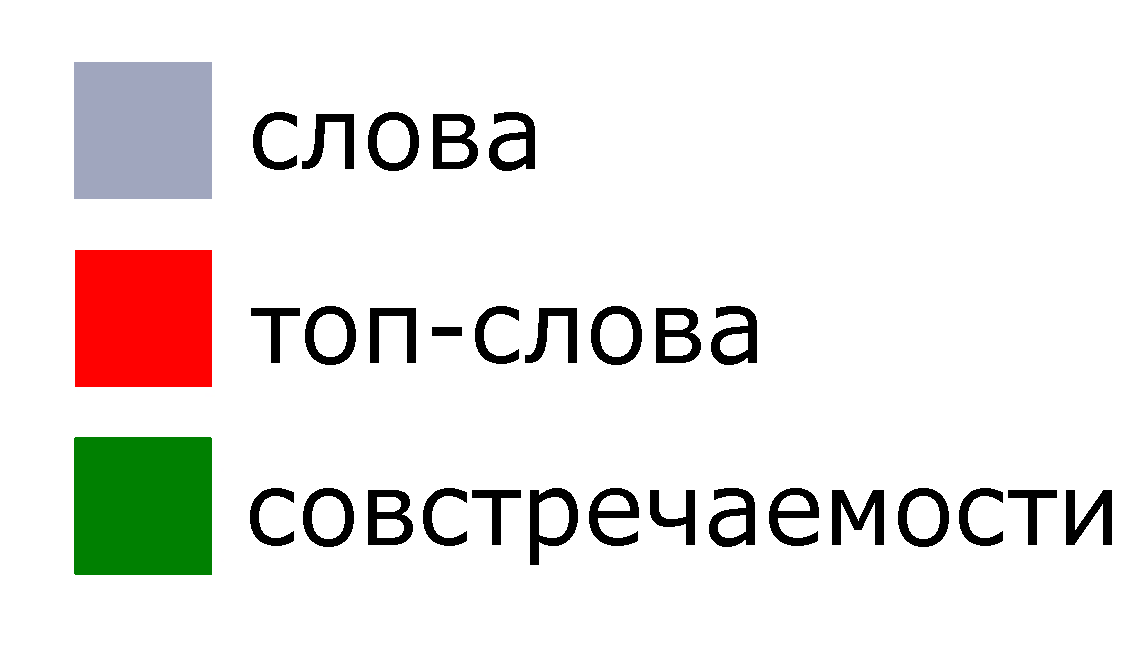
\includegraphics[width=\textwidth]{legend.eps}
  \end{minipage}
  \begin{block}{}
    Десять топовых слов покрывают малую часть всего текста.
    \emph{Совстречаемостей} этих слов (то есть позиций топ\=/слов, когда рядом с ними есть другие топ\=/слова) ещё меньше.
  \end{block}
\end{frame}

%\section{Цель исследования}
\begin{frame}{Цель исследования}
  \begin{block}{Проблема}
    Когерентности по топ\=/словам опираются на заданное количество самых частых слов темы.
    Этот список слов несёт информацию лишь о части тематической модели.\\
    Помимо этого, оценивать интерпретируемость с помощью экспертов дорого и затратно.
  \end{block}
  \begin{block}{Решение}
    Смотреть, как тема распределена по \emph{всем} словам текста.\\
    Считать когерентность темы как среднюю схожесть слов, близко расположенных в тексте.
  \end{block}
\end{frame}


\begin{frame}
  \frametitle{Содержание}
  \tableofcontents
\end{frame}


%\section{Пролог}
%\subsection{Тематическое моделирование}
%\begin{frame}{Тематическое моделирование}
%  Тематическая модель описывает коллекцию документов через \emph{скрытые} темы.
%  \smallskip
%  
%  \begin{itemize}
%    \item $\phi_{wt} \equiv p(w \mid t)$~---~вероятность встретить слово $w$ в теме $t$
%    \item $\theta_{td} \equiv p(t \mid d)$~---~вероятность найти тему $t$ в документе $d$
%  \end{itemize}
%  
%  \begin{figure}[b]
%    \centering
%    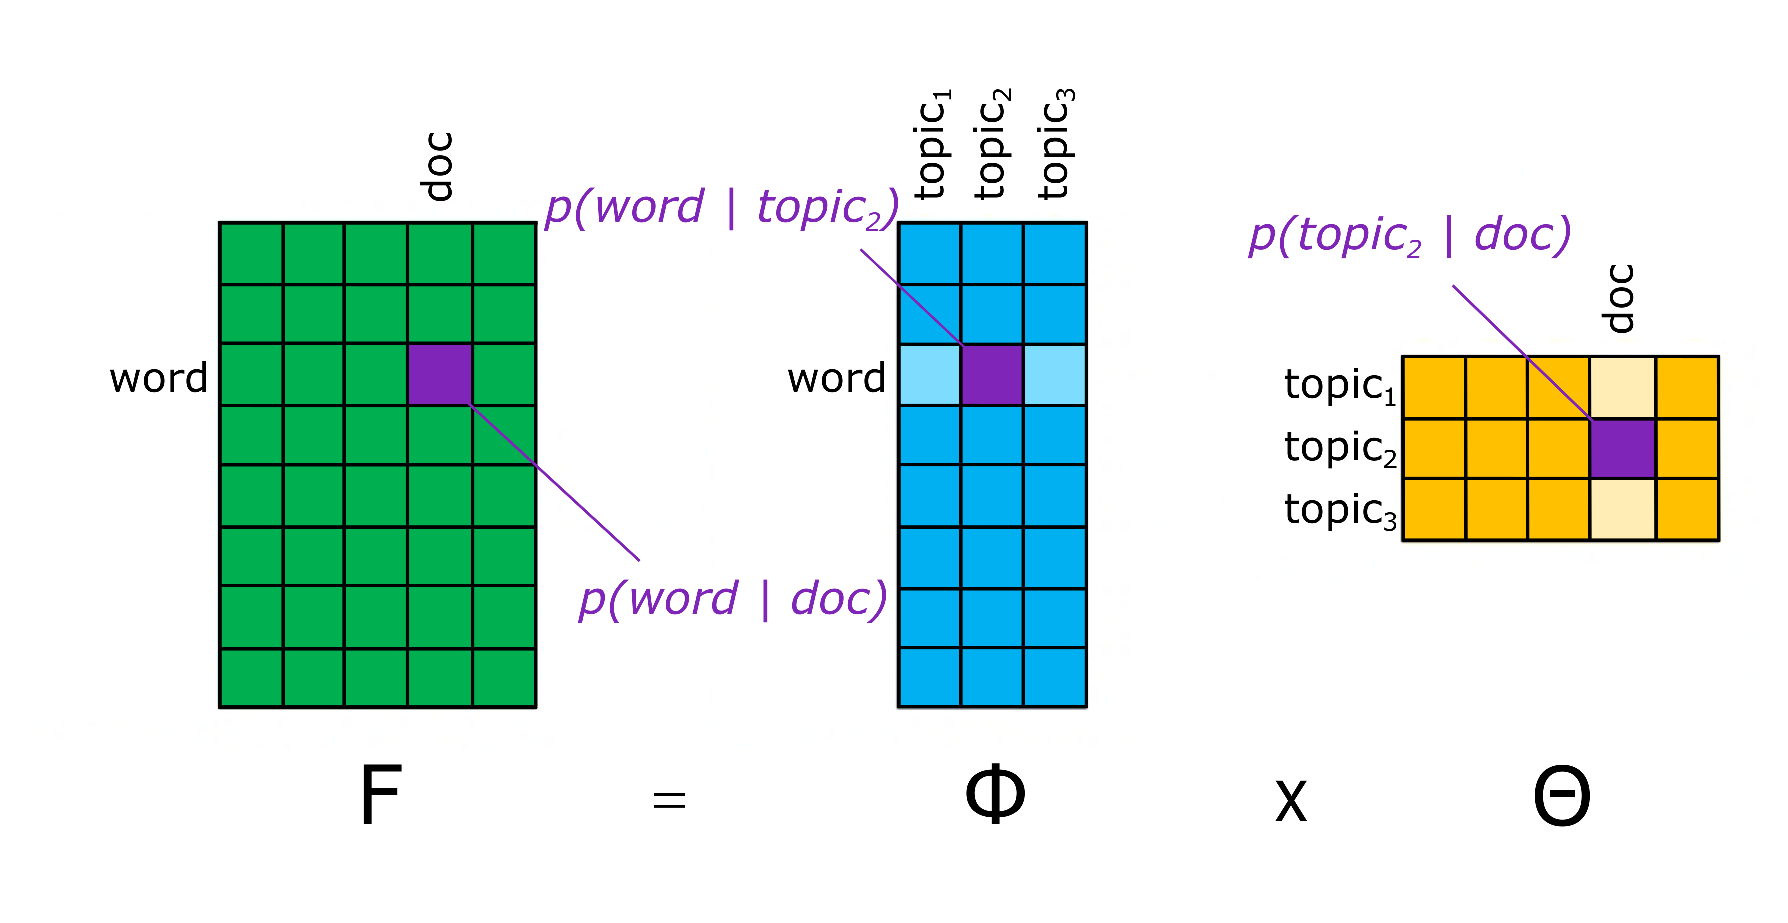
\includegraphics[width=\textwidth]{plsa_matrices.eps}
%  \end{figure}
% \end{frame}



\section{Внутритекстовые когерентности}

\begin{frame}{SemantiC (L2, Cos): Semantic Closeness}
  \begin{block}{Значение}
    Близость близко расположенных в тексте слов темы $t$
  \end{block}
  
  \vspace{-0.6cm}
  
  \begin{table}[]
  %\begin{tabular}{lllll}
  \begin{tabularx}{320pt}{l| *{4}{Y}|}
    %& Group of & astronomers & discovered & a star \\
    & Группа & астрономов & обнаружила & звезду \\
    \begin{tabular}[c]{@{}l@{}}$\begin{matrix}\\ \textit{\textcolor{my-red}{\mbox{Астрономия}}} \\\\
    \textit{\textcolor{my-green}{\mbox{Биология}}} \\\\
    \textit{\textcolor{blue}{\mbox{Музыка}}} \\\\
    \end{matrix}$\end{tabular} & 
    \begin{tabular}[c]{@{}l@{}} 
      $\topicvector{my-red!10}{my-green!33}{blue!66}$
    \end{tabular} & 
    \begin{tabular}[c]{@{}l@{}}
      $\topicvector{my-red!90}{my-green!10}{blue!10}$
    \end{tabular} &  
    \begin{tabular}[c]{@{}l@{}}
      $\topicvector{my-red!45}{my-green!45}{blue!10}$
    \end{tabular} & 
    \begin{tabular}[c]{@{}l@{}}
      $\topicvector{my-red!75}{my-green!10}{blue!55}$
    \end{tabular}
  \end{tabularx}
  \end{table}
  
  Сравниваются пары векторов слов: например $\smalltopicvector{my-red!90}{my-green!10}{blue!10}$ и $\smalltopicvector{my-red!75}{my-green!10}{blue!55}$
\end{frame}


\begin{frame}{SemantiC (Var): Semantic Closeness}
  \begin{block}{Значение}
    Разброс темы $t$ по близко расположенным словам
  \end{block}
    
  \vspace{0.5cm}
  
  \begin{table}[]
  \small
  \begin{tabularx}{1.0\textwidth}{l| *{3}{Y}|*{3}{Y}|}
    & \multicolumn{3}{c|}{Малый разброс} 
    & \multicolumn{3}{c|}{Большой разброс}\\
    \cline{2-7}
    & русский & поэт & Пушкин & Толстой & Рассел & Эйлер \\
    \begin{tabular}[c]{@{}l@{}}$\begin{smallmatrix}\\ \textit{\textcolor{my-red}{Литература}} \\\\
    \textit{\textcolor{my-green}{\mbox{Философия}}} \\\\
    \textit{\textcolor{blue}{\mbox{Математика}}} \\\\
    \end{smallmatrix}$\end{tabular}  &
    \begin{tabular}[c]{@{}l@{}} 
      $\smalltopicvector{my-red!50}{my-green!25}{blue!25}$
    \end{tabular} & 
    \begin{tabular}[c]{@{}l@{}}
      $\smalltopicvector{my-red!90}{my-green!10}{blue!10}$
    \end{tabular} &  
    \begin{tabular}[c]{@{}l@{}}
      $\smalltopicvector{my-red!90}{my-green!10}{blue!10}$
    \end{tabular} &  
    \begin{tabular}[c]{@{}l@{}}
      $\smalltopicvector{my-red!90}{my-green!30}{blue!10}$
    \end{tabular} &  
    \begin{tabular}[c]{@{}l@{}}
      $\smalltopicvector{my-red!10}{my-green!50}{blue!50}$
    \end{tabular} &  
    \begin{tabular}[c]{@{}l@{}}
      $\smalltopicvector{my-red!10}{my-green!10}{blue!90}$
    \end{tabular}  
  \end{tabularx}
  \end{table}
\end{frame}


\begin{frame}{FoCon: Focus Consistency}
  \begin{block}{Значение}
    Как сильно изменяется тема среди смежных слов
  \end{block}
  
  \medskip
  
  Метод не привязан к теме, он сразу даёт значение когерентности для \emph{тематической модели} как целого.
  
  \begin{figure}[h]
    \centering
    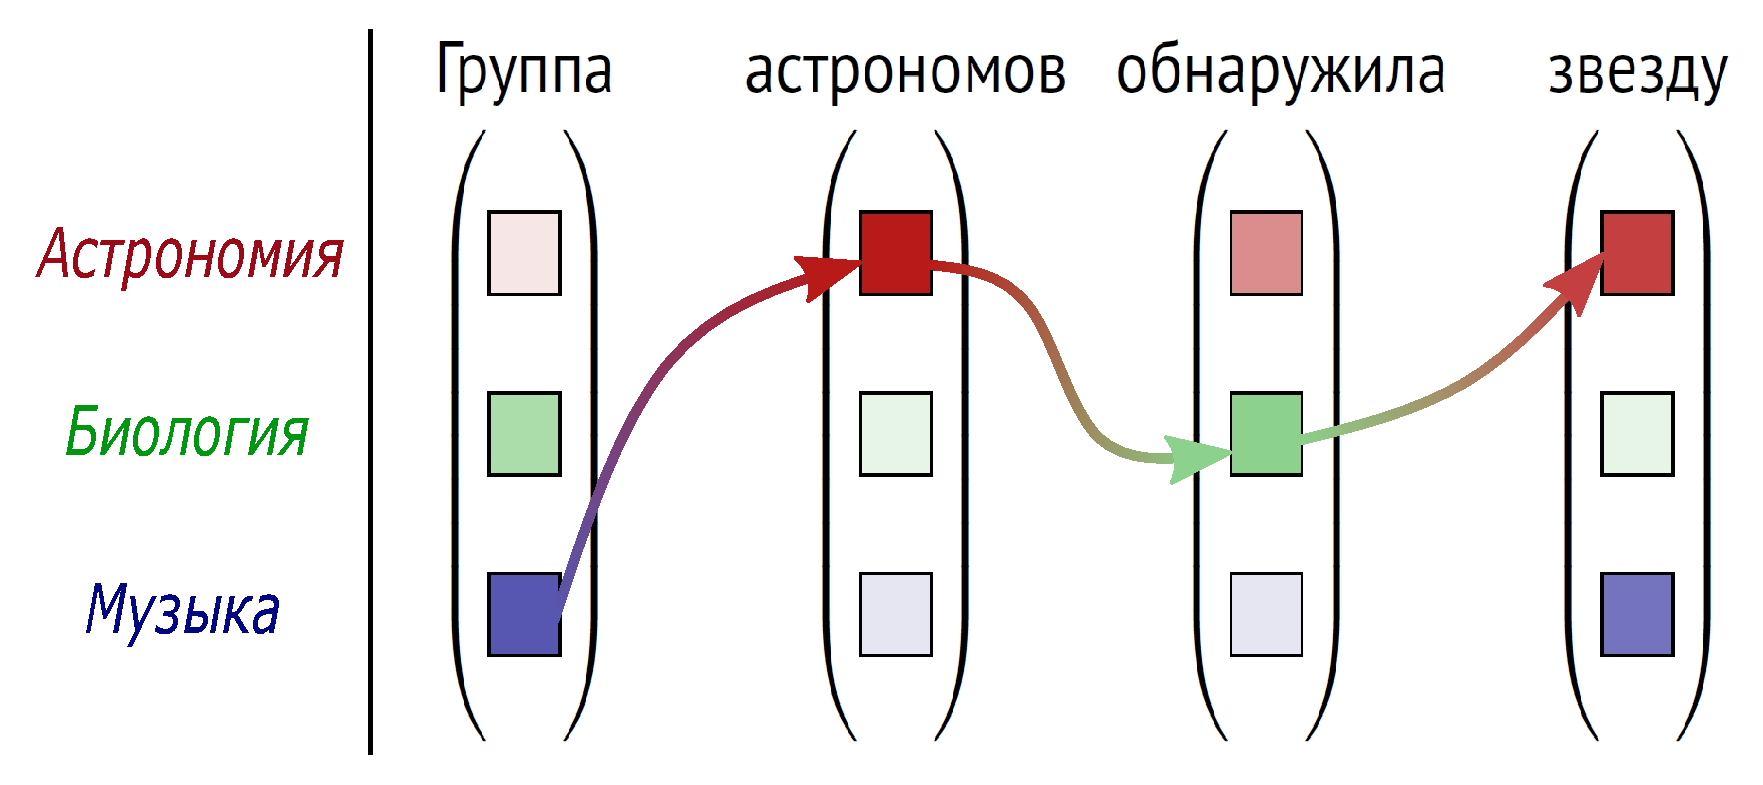
\includegraphics[width=1.0\textwidth, height=0.45\textheight]{astronomers_focon.eps} % .eps image is wrong scaled
  \end{figure}
\end{frame}


\begin{frame}{TopLen: Topic Length}
  \begin{block}{Значение}
    Средняя длина темы внутри текста
  \end{block}
  
  \medskip
  
  Считает слова темы $t$, штрафуя, когда встречается слово другой темы.
  
  \vspace{0.5cm}
  
  \begin{block}{Пример для темы $t = \mbox{<<Чёрные дыры>>}$}
    \noi
    $\mbox{Группе}\ \underbrace{\mbox{\textcolor{my-pink}{астрономов}}\ \mbox{удалось}}_{l_1=2}\ \mbox{обнаружить}\ \underbrace{\mbox{\textcolor{my-pink}{звезду}}, \mbox{обращающуюся}}_{l_2=2}$\\
    $\mbox{вокруг}\ \underbrace{\mbox{\textcolor{my-red}{чёрной}}\ \mbox{\textcolor{my-red}{дыры}}\ \mbox{на}\ \mbox{рекордно}\ \mbox{близком}}_{l_3=4}\ \mbox{расстоянии}.$
  \end{block}
\end{frame}


\section{Полуавтоматическая оценка качества функций когерентности}

\subsection{Полусинтетический датасет}

\begin{frame}{Полусинтетический датасет}
  \begin{block}{Гипотеза}
    Все тексты сегментированы.
    Но позиции сегментов не известны
  \end{block}
  
  $2000$ \emph{монотематических} статей <<ПостНауки>>\footnote[frame]{https://postnauka.ru} разрезаются на сегменты одинаковой длины и сшиваются в новые документы.
    
  \begin{figure}[h]
    \centering
    \includegraphics[width=0.6\textwidth, height=0.45\textheight]{pn_gen_diagram.eps}
    \caption*{Документ из двух сегментов: про <<социологию>> и <<медицину>>}
  \end{figure}    
\end{frame}


\begin{frame}{Полусинтетический датасет}
  \begin{block}{}
    Чем лучше функция когерентности, тем лучше она должна описывать способность тематической модели угадывать сегментную структуру текста
  \end{block}
  
  \begin{columns}
  \column{0.5\textwidth}
  
  Для каждого слова в полусинтетическом датасете известно, к какой теме оно относится
  
  \column{0.5\textwidth}
  
  \begin{figure}[b]
    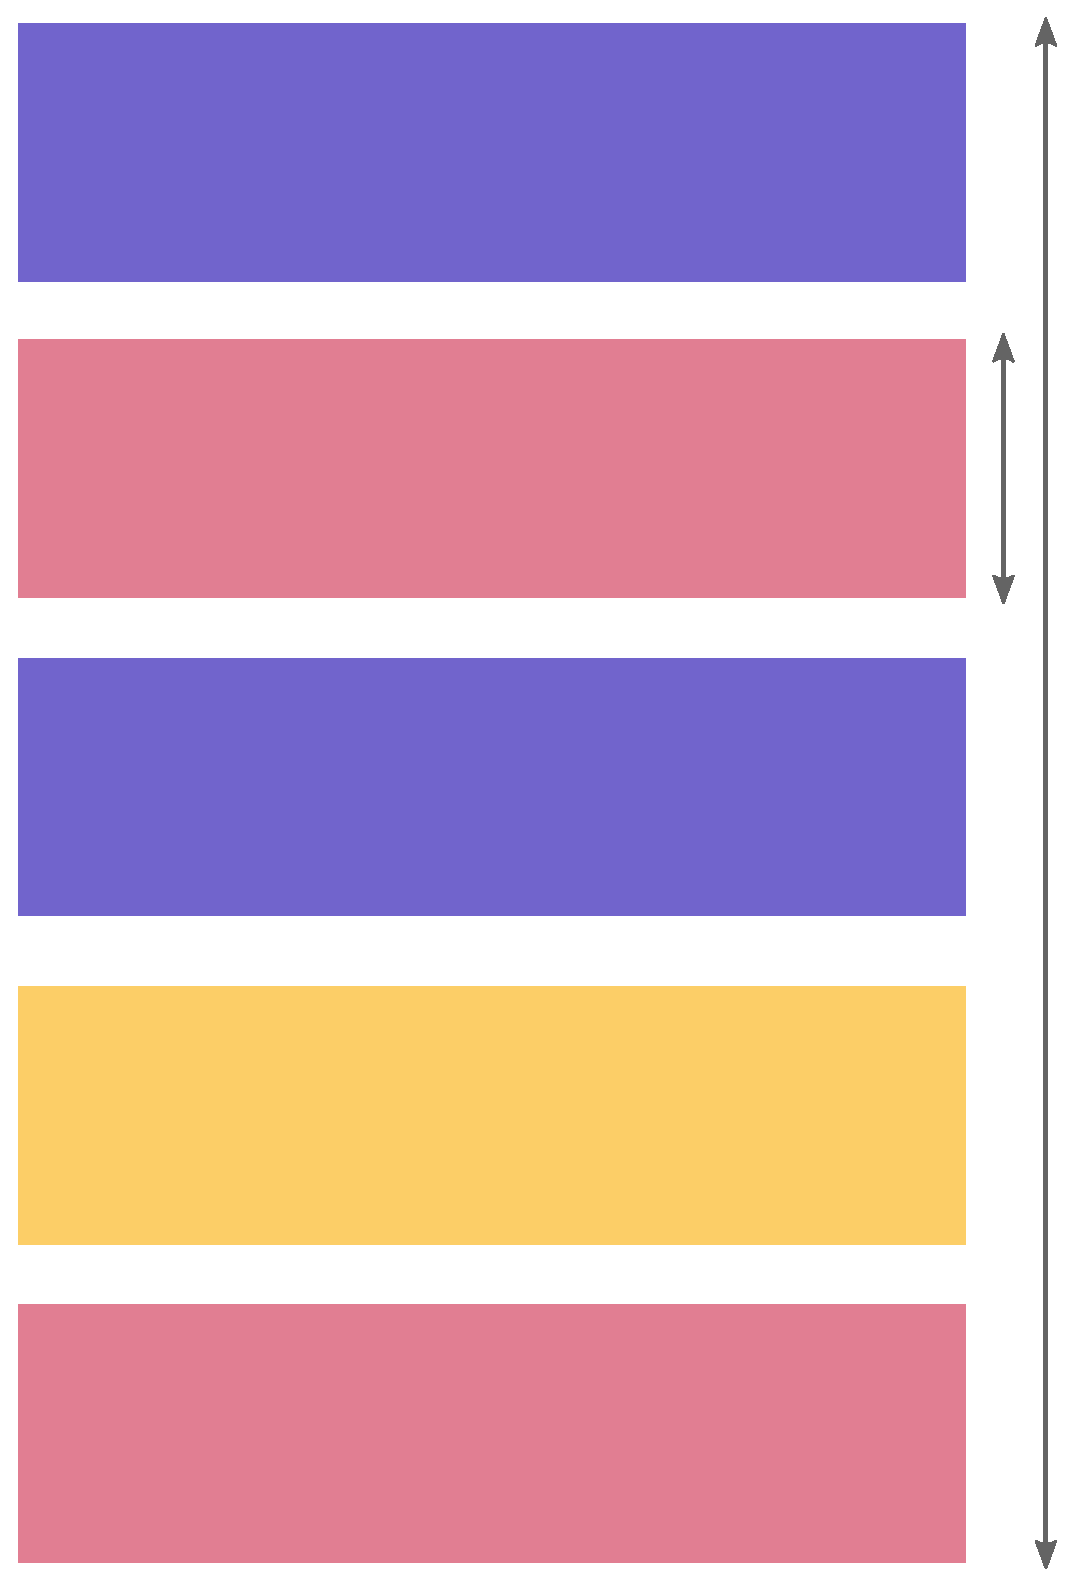
\includegraphics[width=\linewidth, height=0.5\textheight]{dataset.eps} % scale=0.20
  \end{figure}
  \end{columns}
\end{frame}

	
\subsection{Качество сегментации}


\begin{frame}{Качество сегментации: Soft}
  \begin{block}{}
    Сумма $p(t \mid d, w)$ по всем словам в сегментах темы $t$
  \end{block}
  
  \vspace{1.2em}
  
  \begin{figure}[h]
    \centering
    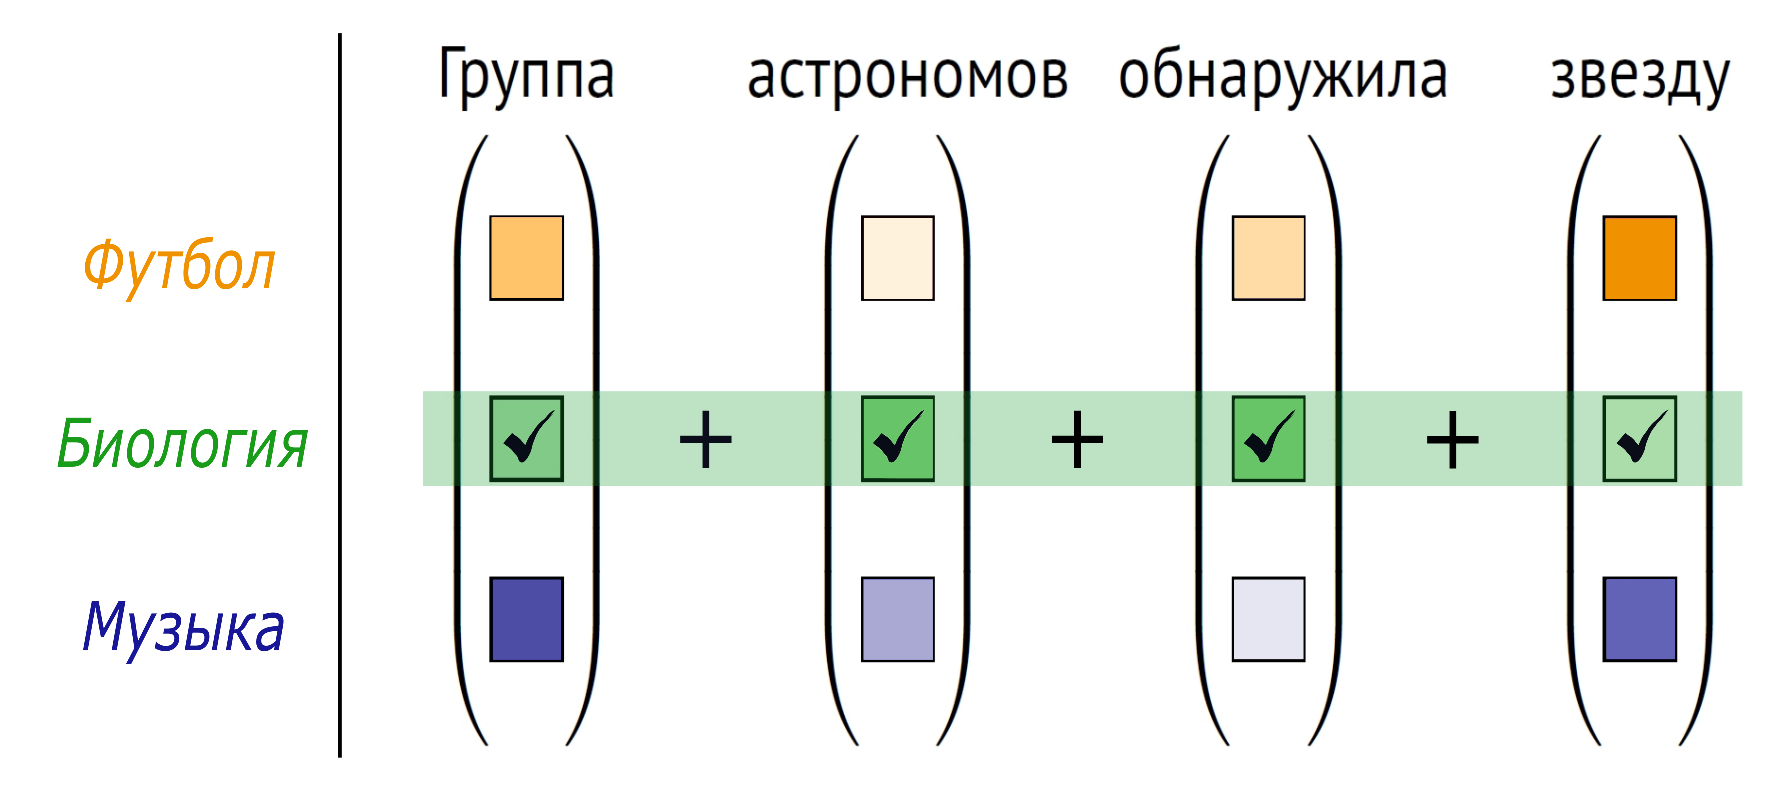
\includegraphics[width=1.0\textwidth, height=0.45\textheight]{astronomers_soft.eps} % .eps image is wrong scaled
  \end{figure}
\end{frame}


\begin{frame}{Качество сегментации: Hard}
  \begin{block}{}
    Количество совпадений между темой, предсказываемой моделью $\argmax_\tau p(\tau \mid d, w)$, и действительной темой среди слов в сегментах темы $t$
  \end{block}
  
  \begin{figure}[h]
    \centering
    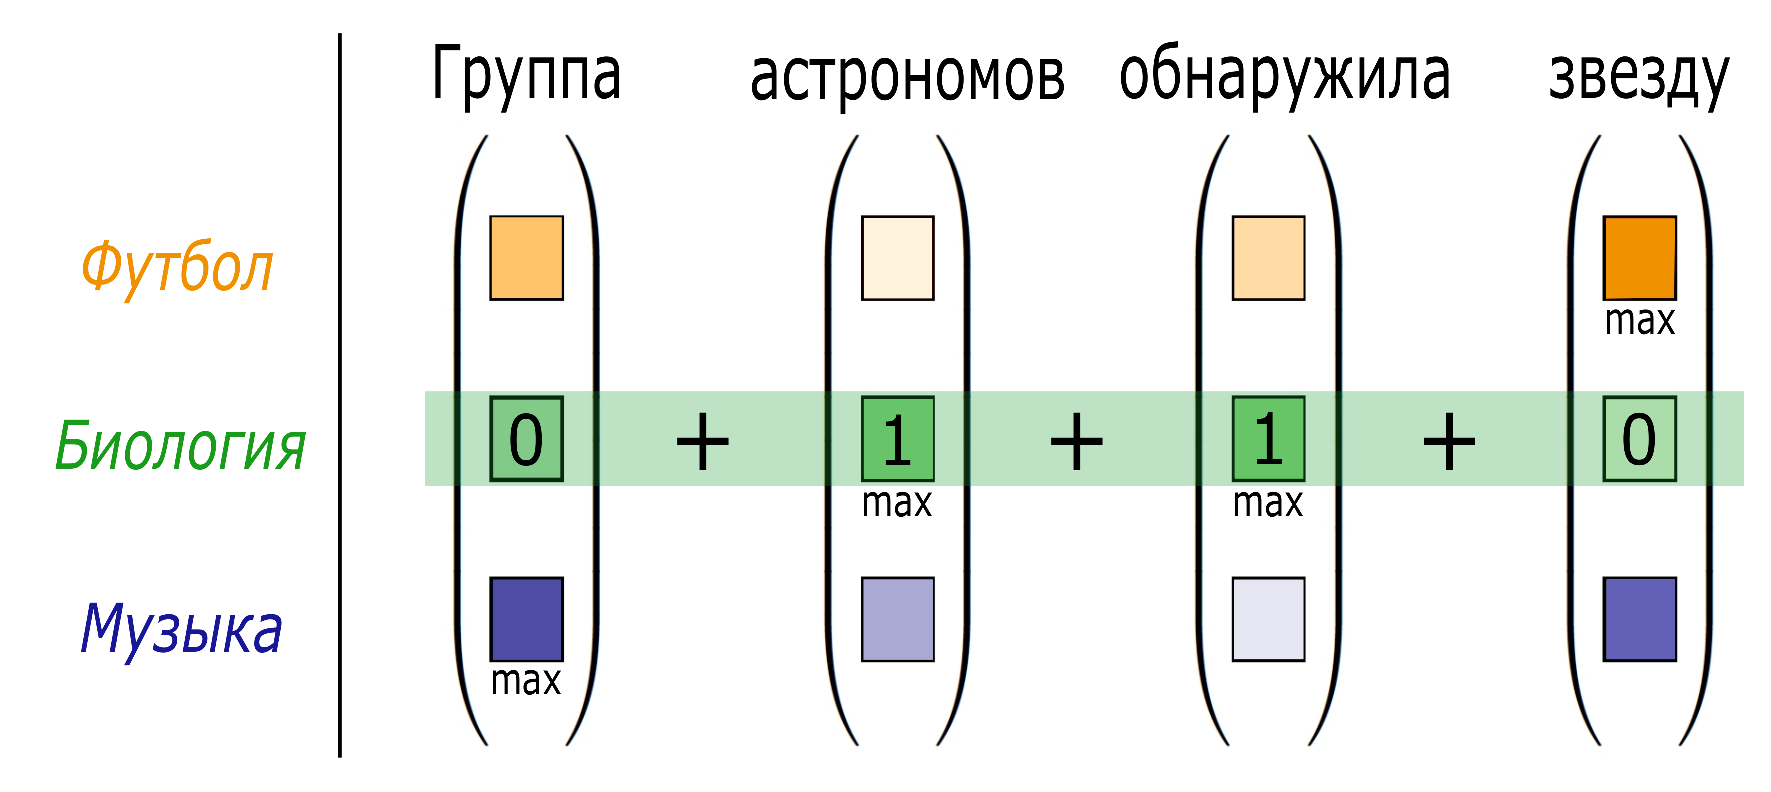
\includegraphics[width=1.0\textwidth, height=0.45\textheight]{astronomers_strict.eps} % .eps image is wrong scaled
  \end{figure}
\end{frame}


\section{Эксперименты}


\begin{frame}{Недостаток подхода с помощью топ\=/слов}
  \begin{block}{}
    Когерентности по топ\=/словам могут игнорировать более 98\% слов текста коллекции документов
  \end{block}
  
  \bigskip
  
  \begin{table}[h]
    \centering
    \captionsetup{justification=centering}
    
    \begin{tabular}{lcc}
      % {} & ПостНаука, \%\\% & Википедия, \%\\
      \toprule
      Min & $0.016$\\% & 0.0065\\
      Mean & $0.062$\\% & 0.036\\
      Max & $0.28$\\% & 0.11\\
      \midrule
      Total & $\mathbf{1.2}$\\% & \textbf{1.7}
      \bottomrule
    \end{tabular}
    
    \caption*{Часть корпуса (\%), которая занята совстречаемостями десяти топовых слов для тем <<ПостНауки>>}
  \end{table}
\end{frame}


\begin{frame}{Спирмановские корреляции между когерентностями и качестами сегментации}
  \begin{block}{}
    Ряд тематических моделей: от <<хорошей>> модели коллекции <<ПостНаука>> до плохой модели, матрица $\Phi$ которой взята из некоторого вероятностного распределения
  \end{block}
  \begin{table}[t]
    \begin{tabular}{lr}
      Coh & Corr\\
      \midrule
      Newman & $0.75$\\
      Mimno & $0.96$\\
      \midrule
      SC L2 & $0.92$\\
      SC Cos & $-0.97$\\
      SC Var & $\mathbf{1.00}$\\
      TopLen & $\mathbf{1.00}$\\
      FoCon & $\mathbf{1.00}$\\
      \bottomrule
    \end{tabular}
    ~
    \begin{tabular}{lr}
      Coh & Corr\\
      \midrule
      Newman & $0.80$\\
      Mimno & $0.94$\\
      \midrule
      SC L2 & $0.70$\\
      SC Cos & $-0.97$\\
      SC Var & $\mathbf{1.00}$\\
      TopLen & $\mathbf{1.00}$\\
      FoCon & $\mathbf{1.00}$\\
      \bottomrule
    \end{tabular}
    ~
    \begin{tabular}{lr}
      Coh & Corr\\
      \midrule
      Newman & $0.85$\\
      Mimno & $0.97$\\
      \midrule
      SC L2 & $0.59$\\
      SC Cos & $-0.96$\\
      SC Var & $\mathbf{1.00}$\\
      TopLen & $\mathbf{1.00}$\\
      FoCon & $\mathbf{1.00}$\\
      \bottomrule
    \end{tabular}
    \centering
    \captionsetup{justification=centering}
    \caption*{
      Результаты для сегментов с размерами $50$, $200$ и $400$ слов и $5$ темами в каждом документе
    }
  \end{table}
\end{frame}


\begin{frame}{Когерентности и качества сегментации как функции качества тематической модели}
  % dataset $\sgm=200,\ \thm=5$
  
  \begin{figure}[h]
    \begin{subfigure}[t]{0.48\textwidth}
      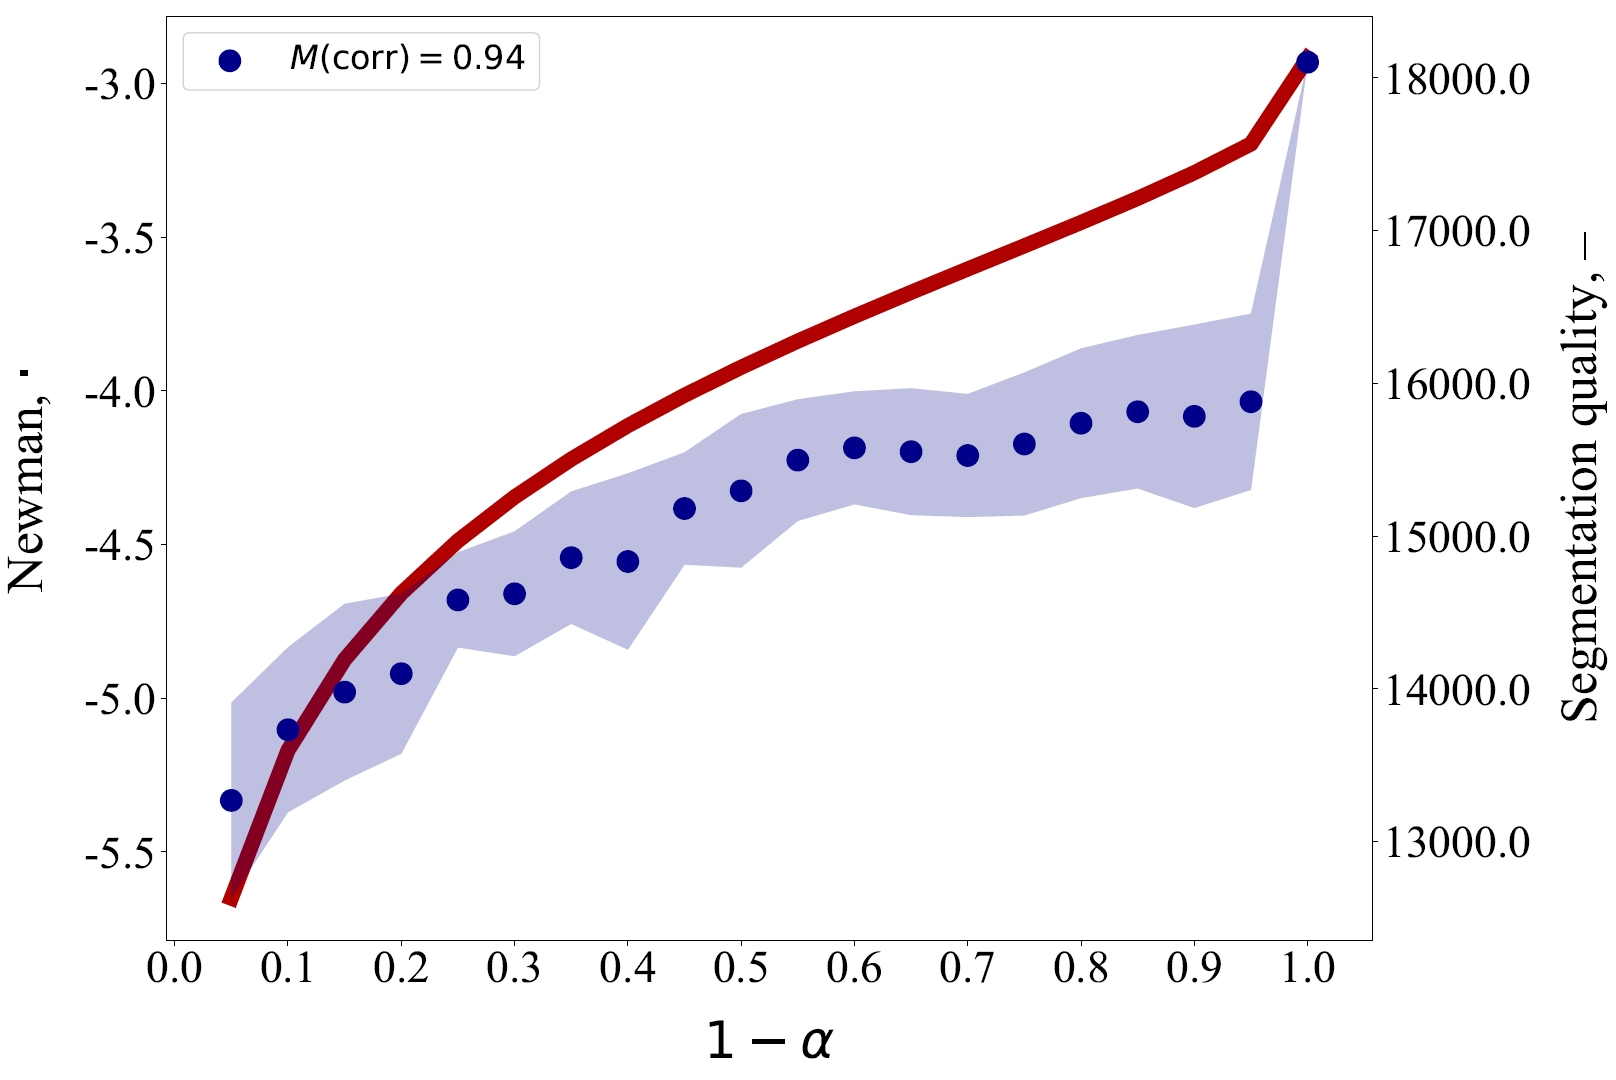
\includegraphics[width=\linewidth]{newman-iteration.jpg}
    \end{subfigure}
    ~
    \begin{subfigure}[t]{0.48\textwidth}
      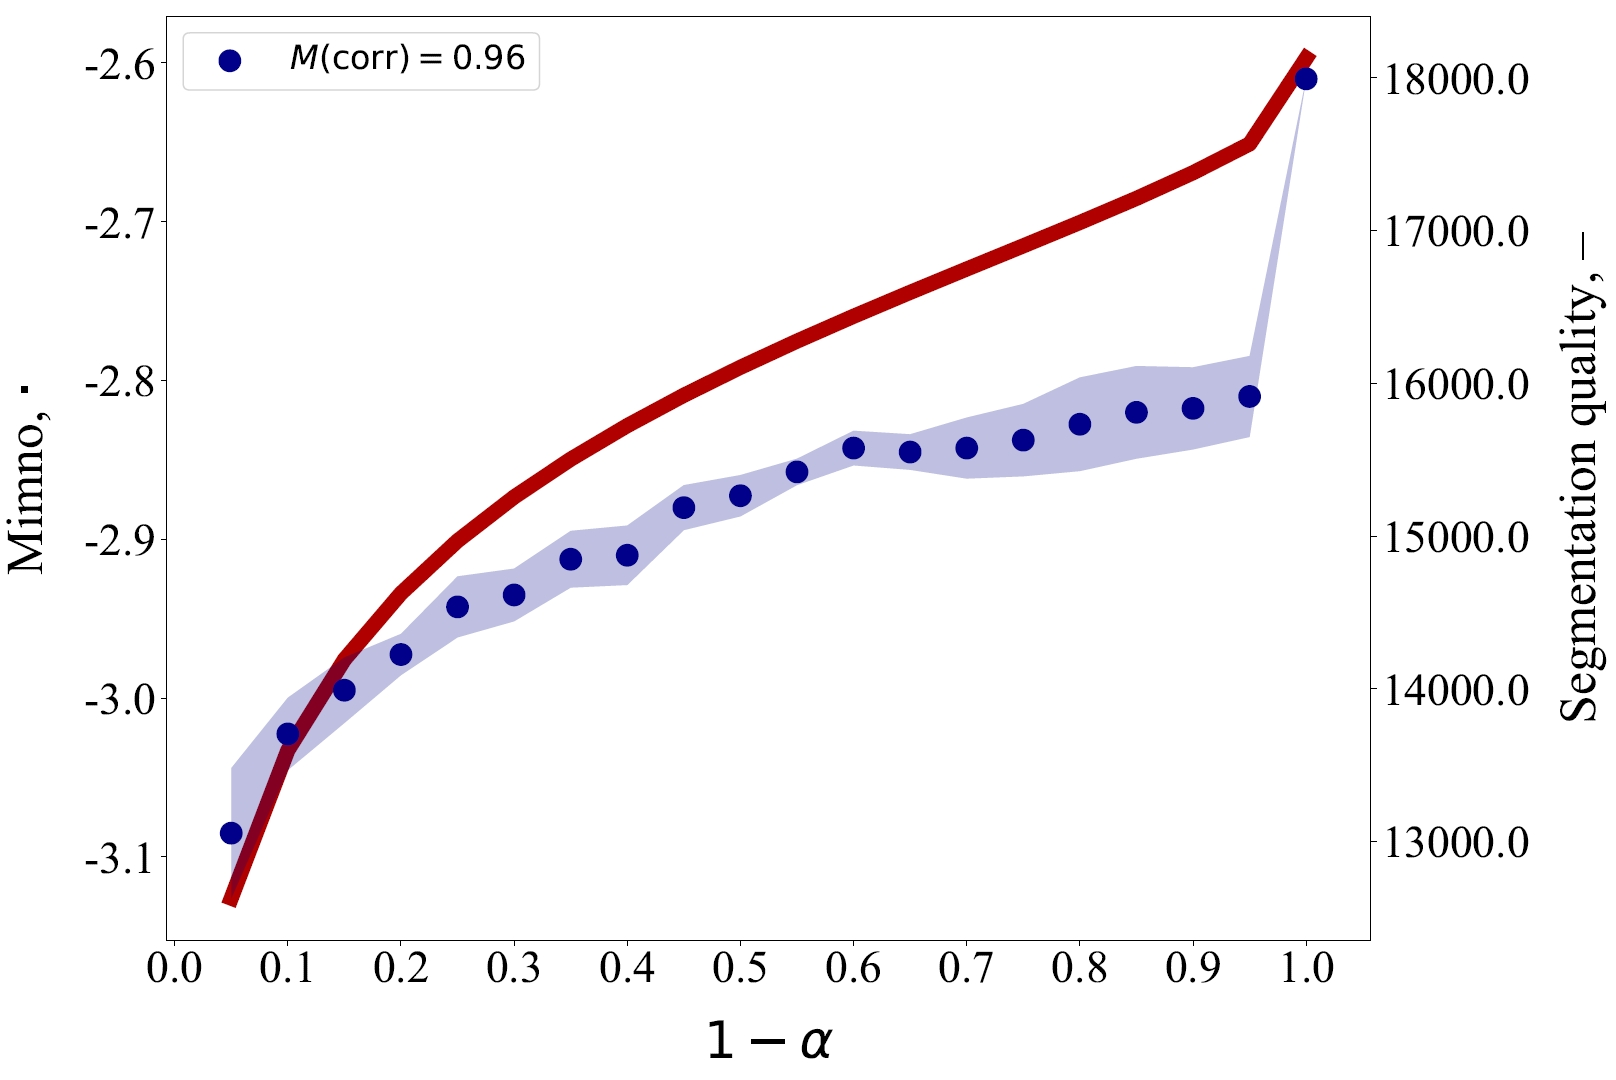
\includegraphics[width=\linewidth]{mimno-iteration.jpg}
    \end{subfigure}
    %%
    \begin{subfigure}[t]{0.48\textwidth}
      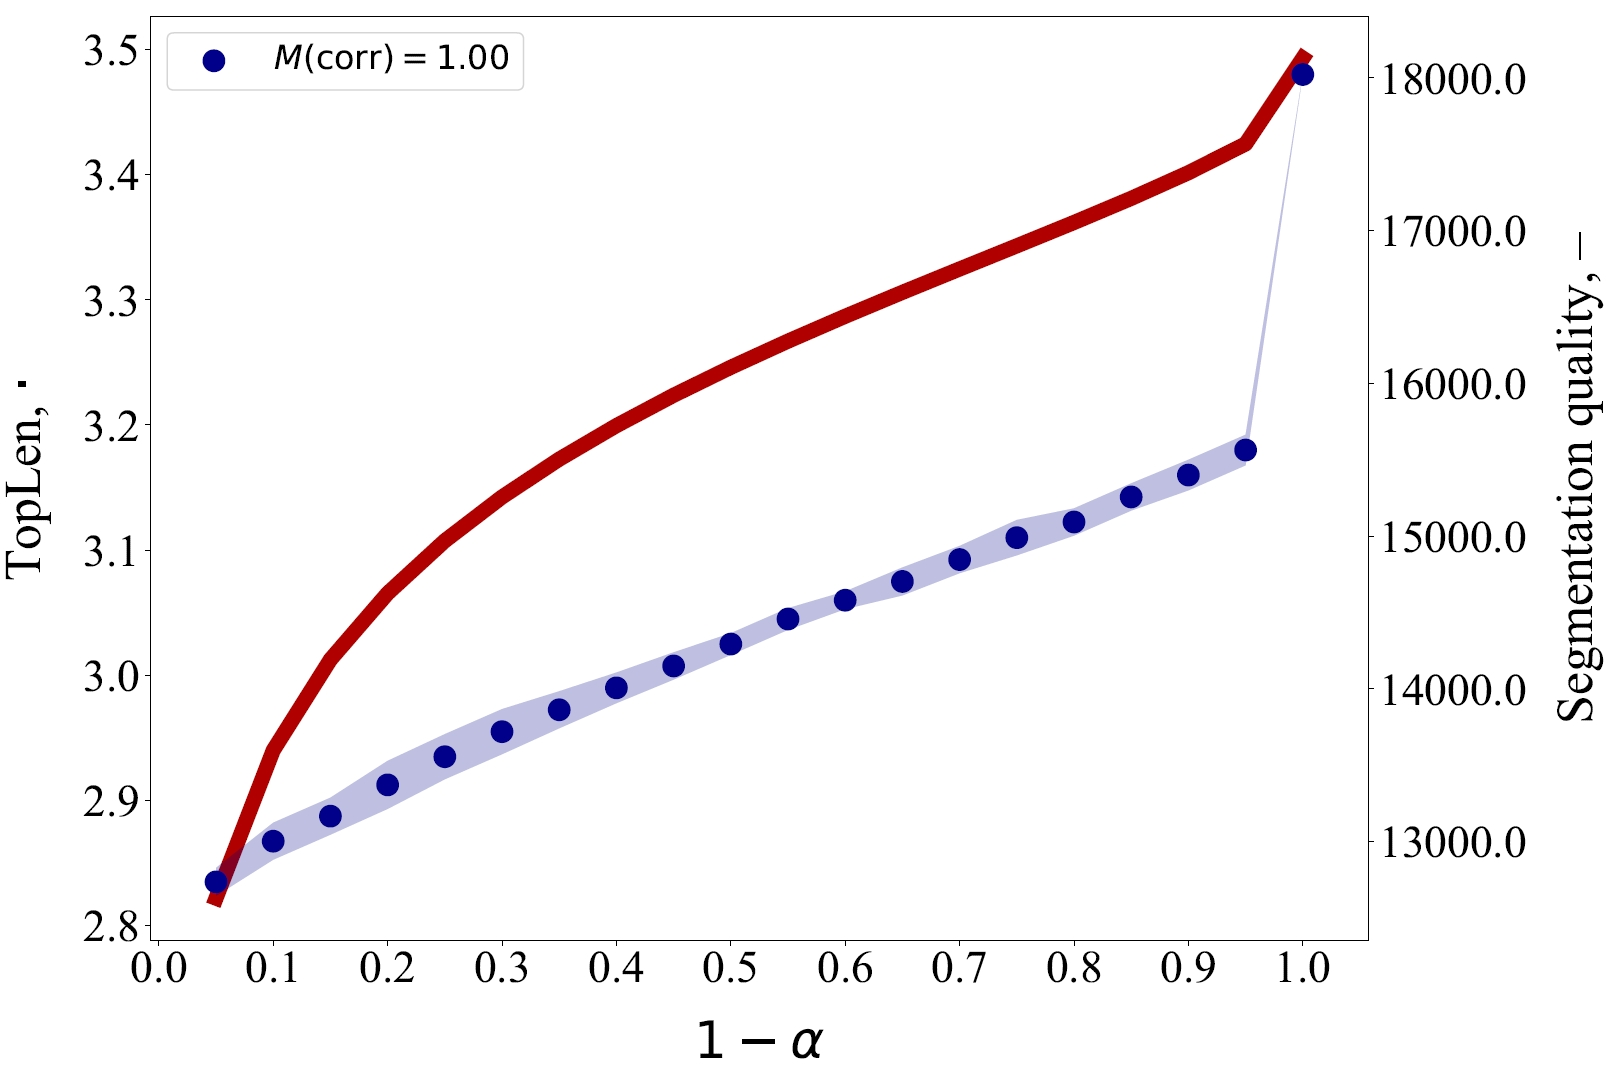
\includegraphics[width=\linewidth]{toplen-iteration.jpg}
    \end{subfigure}
    ~
    \begin{subfigure}[t]{0.48\textwidth}
      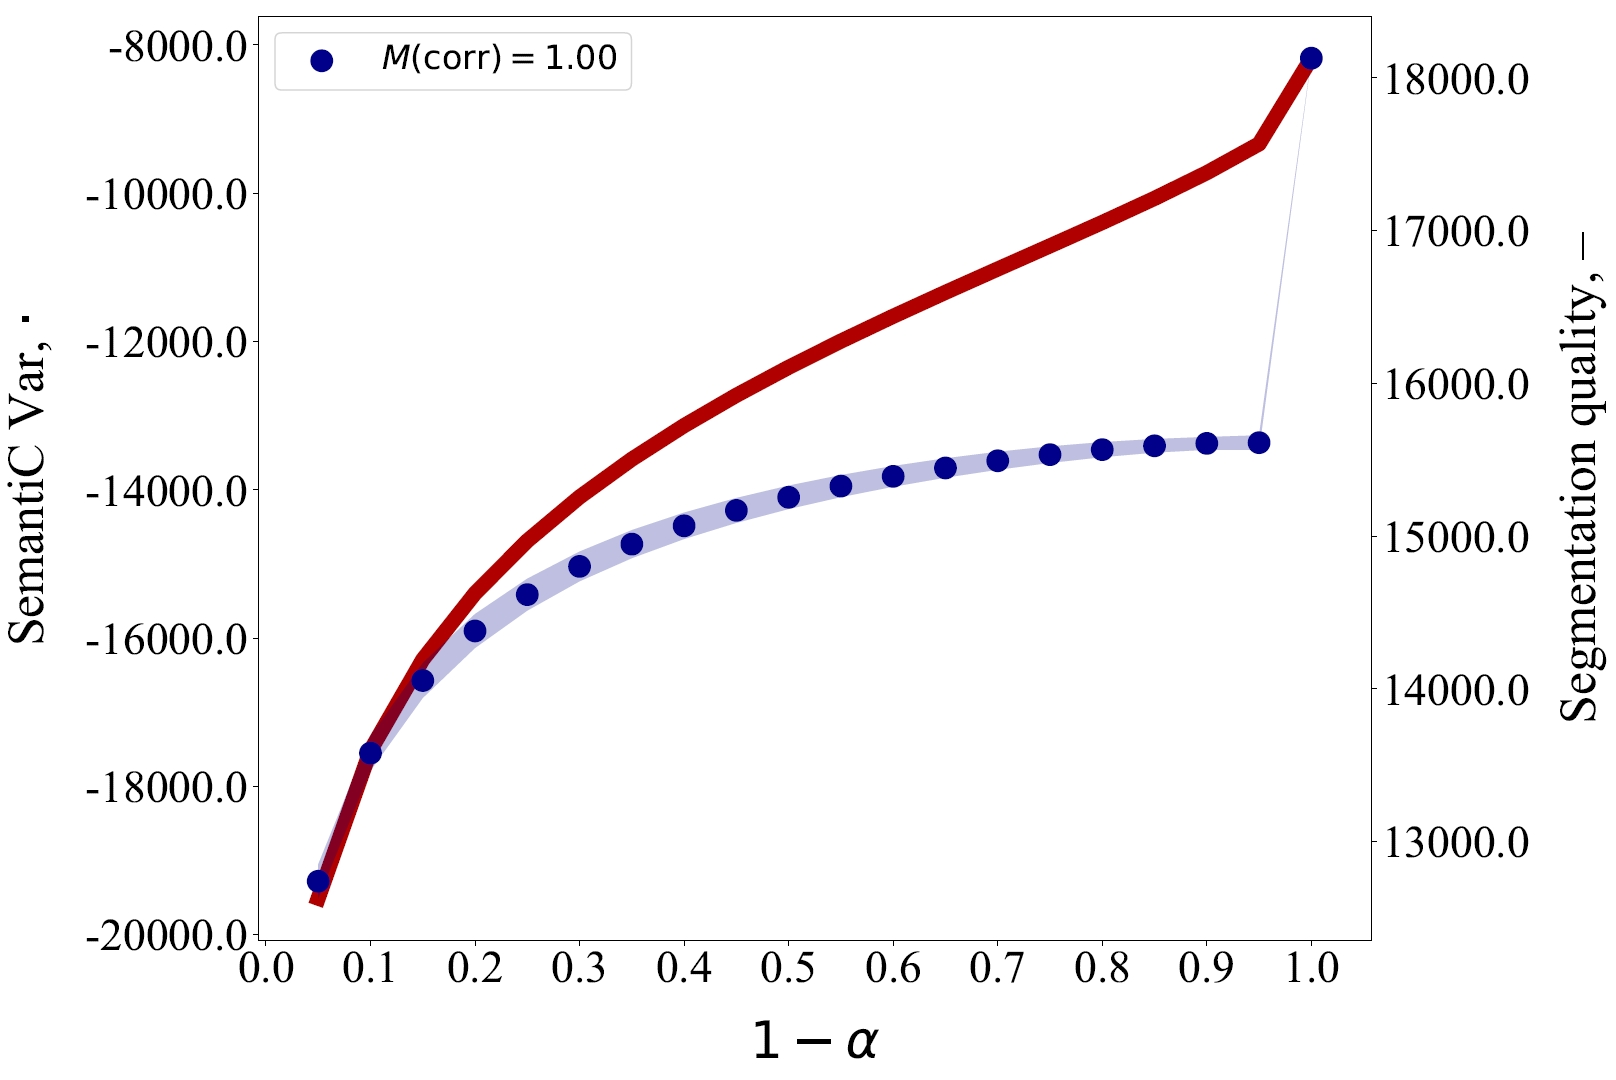
\includegraphics[width=\linewidth]{semantic_var-iteration.jpg}
    \end{subfigure}
  \end{figure}
\end{frame}


\begin{frame}{Результаты}
  \begin{itemize}\setlength\itemsep{0.5cm}
  \item Проиллюстрирован недостаток когерентностей по топ-словам: покрытие лишь малой части текстовой коллекции.

  \item Предложен полуавтоматический метод оценки качества функций когерентности: по корреляции с качеством сегментации полусинтетического текста тематическими моделями.

  \item Представлены методы \emph{внутритекстовой} когерентности.
    По предложенной функции оценки качества некоторые новые методы показывают лучшие результаты, чем когерентности по топ\=/словам.
  \end{itemize}
\end{frame}
\end{document}